%!TEX root = ../thesis.tex

% \pagebreak[4]
% \hspace*{1cm}
% \pagebreak[4]
% \hspace*{1cm}
% \pagebreak[4]

\chapter{Outils multidimensionnels}

\graphicspath{{Chapter1/Chapter1Figs/PNG/}{Chapter1/Chapter1Figs/PDF/}{Chapter1/Chapter1Figs/}}

Ce chapitre propose un état de l'art sur les différents outils de déformation
spatiale d'après le travail de \cite{GB08}. Les outils présentés sont
utilisables aussi bien dans $\mathbb{R}^2$ que dans $\mathbb{R}^3$, mais dans
ce chapitre nous considèrerons des déformations affectant l'espace
$\mathbb{R}^3$

La déformation spatiale est une technique de déformation permettant de
modifier la position des sommets d'un objet virtuel au travers de la
modification de son espace ambiant. Cette déformation est appliquée au travers
de la manipulation d'un \textit{outil}. Un utilisateur va interagir avec un
outil (en modifiant la position de ses sommets), et cet outil va modifier la
position des points de l'espace. Dans la suite du rapport, nous appelons
\textit{objet} un objet virtuel auquel nous appliquons une déformation, et
\textit{point de l'espace} un sommet du objet à déformer.

Ces outils ont différentes caractéristiques, comme par exemple leur dimension
(point, courbe, surface, volume), la zone de l'espace qu'ils déforment (locale
ou globale) ou encore leur résolution (nombre de points de contrôle qui les
composent). On dit qu'une déformation est globale lorsque le déplacement d'un
sommet de l'outil influe sur l'ensemble des points de l'espace.

En pratique, la déformation d'un objet se décompose en 3 étapes :
\begin{enumerate}

\item Construction de l'outil permettant la déformation

\item Association des points de l'espace à l'outil (\textit{temps
d'association})

\item Déformation de l'objet par invariance de l'association (\textit{temps de
déformation})

Les explications ci-dessous se concentrent sur la partie association des
points de l'espace à l'outil.

\end{enumerate} 

\section{Déformation à base de volumes}

Les déformations à base de volumes sont définies à partir d'une grille 3D de
points de contrôle. Ces points peuvent être considérées comme des poignées que
l'on peut déplacer et qui vont modifier la position des points de l'espace.

\begin{itemize}

\item{\textbf{Déformation de forme libre de Bézier :}} \cite{SP86} ont eu
l'idée de lier la déformation d'un volume paramétrique à l'espace contenu à
l'intérieur de ce volume. Mathématiquement, il s'agit d'une extension directe
des courbes de Bézier au cas 3D. Ils ont utilisé les polynômes de Bernstein
pour définir le volume. Ce modèle, attribuant une forme parallépipédique au
volume (Figure \ref{SURPar}), permet d'obtenir une paramétrisation des
coordonnées des points de l'espace presque automatiquement. Cette technique
déforme l'espace de façon globale. Les volumes paramétriques souffrent des
mêmes problèmes que leurs homologues de dimensions inférieures (surface et
courbes paramétriques), à savoir le manque de contrôle local.

\begin{figure}[!ht]
  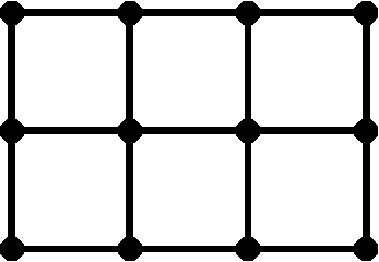
\includegraphics{chapter1-bezierPara-pstricks}
  \caption[Volume de Bézier parallélépipédique] {Vue en coupe d'un volume de
  Bézier parallélépipédique.}
  \label{SURPar}
\end{figure}

\item{\textbf{Déformation de forme libre avec contrôle local :}} Pour corriger
le problème de contrôle local, une solution naïve consiste à rajouter des
points de contrôle afin de réduire l'impact de chacun d'entre eux sur l'espace
à déformer. Mais cette technique augmente la résolution du volume paramétrique
et ainsi sa complexité en temps de calcul. Une autre solution est d'utiliser
des fonctions définies par morceaux. \cite{GP89} et \cite{Com89} ont choisi de
travailler avec des B-splines car elles sont définies naturellement par
morceaux. Ce choix rend la déformation locale.

\item{\textbf{Déformation de forme libre avec outil non parallélépipédique :}}
Les déformations de forme libre ont une grosse limitation, celle de la forme
de l'outil. En effet, comme les volumes de déformations sont uniquement
composés de cubes alignés sur les axes du repère de l'espace, la forme globale
correspond à un pavé. Par conséquent, il n'est pas possible d'obtenir un outil
qui épouse la forme de l'objet à déformer. \cite{Coq90} a donc proposé une
version étendue des déformations de forme libre, en permettant la modification
de la position des points de contrôle avant l'étape d'association. Le calcul
des coordonnées des points de l'espace par rapport à l'outil n'est donc plus
trivial, il devient beaucoup plus coûteux. \cite{BBT97} ont proposé de
considérer des volumes de Bézier tétraédriques (Figure \ref{SURTet}) tandis
que \cite{MJ96} se sont plutôt intéressés aux volumes de subdivision de
topologie quelconque.

\begin{figure}[!ht]
	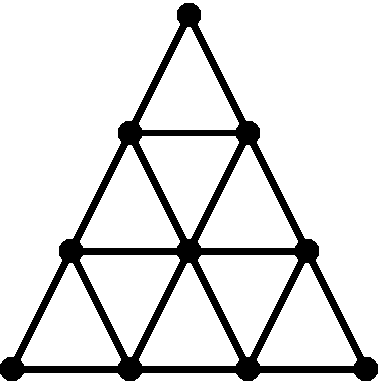
\includegraphics{chapter1-bezierTetra-pstricks}
  \caption[Volume de Bézier tétraédrique] {Vue en coupe d'un volume de
  Bézier tétraédrique.}
  \label{SURTet}
\end{figure}

\end{itemize}

\section{Déformation à base de surfaces} 

La difficulté des déformations à base de surfaces réside dans la manière
d'attacher les points de l'espace à une surface.

\begin{itemize}

\item{\textbf{Carreau paramétrique :}} \cite{JLQ96} ont été les premiers à
proposer une solution, celle d'utiliser un carreau B-spline sur lequel sont
projetés les points de l'espace, le long de la normale au plan du carreau,
dans l'espace paramétrique du carreau. Ainsi pour déformer l'espace,
l'utilisateur déplace les différents points de contrôle. Les points de
l'espace sont repositionnés grâce à leurs coordonnées paramétriques
(précédemment calculées) et "reprojetées" le long de la normale au carreau
déformé. De même que pour les volumes paramétriques, cette technique déforme
l'espace de façon globale.

\item{\textbf{Surface étoilée :}} Un polyèdre de forme étoilée est un polyèdre
contenant, en son intérieur, une région qu'on appelle le \textit{noyau}. On
définit le noyau d'un polyèdre comme étant la région depuis laquelle un rayon
émis dans n'importe quelle direction n'intersecte le bord du polyèdre qu'une
seule fois (Figure \ref{SUReto}, représenté en 2D). Cette propriété est utile
dans le domaine de la déformation car elle permet d'obtenir une unique
paramétrisation en coordonnées polaires des points de l'espace, comme proposé
par \cite{JL00}. Cette technique déforme aussi l'espace de façon globale.

 \begin{figure}[!ht]
  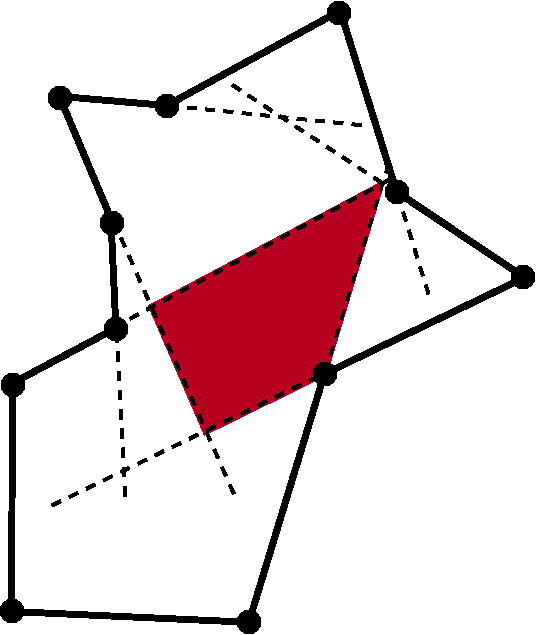
\includegraphics[scale=0.5]{chapter1-noyau-pstricks}

  \caption[Noyau d'un polygone] {En rouge le noyau d'un polygone de forme
étoilée représenté par son bord, en noir (en 2D). Les points de contrôle sont
représentés par les disques noirs.}

  \label{SUReto}
 \end{figure}

\item{\textbf{Maillage triangulaire :}} Une autre idée est d'utiliser un
maillage triangulaire simple pour appliquer des déformations aux points de
l'espace. \cite{KO03} ont été les premiers à utiliser ce genre d'outil. Ils
proposent que les triangles du maillage contribuent à déformer une zone
sphérique autour de chacun d'entre eux. Les triangles définissent des
coordonnées paramétriques pour les points de l'espace se trouvant dans leur
zone d'influence, en fonction de leur distance à chacun des triangles. La
position des points de l'espace se trouvant à l'intersection de plusieurs
zones d'influence résultent d'une moyenne pondérée des coordonnées calculées
par rapport à chaque triangle. L'avantage de cette technique est de permettre
une configuration assez générale des triangles (non nécessairement connexes),
à partir du moment où ceux-ci ne sont pas dégénérés (les triangles doivent
être composés de 3 sommets linéairement indépendants). La déformation
engendrée par le déplacement d'un sommet d'un triangle est locale et définie
par la zone d'influence de ce triangle.

\item{\textbf{Cage :}} La cage est l'outil surfacique le plus utilisé ces
dernières années en terme de déformation spatiale. Son utilisation s'est
développée suite aux travaux de \cite{JSW05} et de \cite{FKR05} qui ont
utilisé les \textit{Mean Value Coordinates} présentées par \cite{Flo03} et
\cite{FKR05}. Un maillage surfacique triangulaire quelconque est créé, et
définit une position paramétrique des points de l'espace par rapport aux
positions des points de contrôle de la cage. Cette méthode est détaillée dans
le prochain chapitre.

\end{itemize}

\section{Déformation à base de courbes} 

\begin{itemize}

\item{\textbf{Déformation de De Casteljau généralisée :}} \cite{CR94} ont
introduit une méthode de déformation à base de courbe qui peut-être vue comme
une déformation de forme libre de Bézier limitée. L'idée est d'associer les
points de l'espace autour de la courbe aux points de contrôle de la courbe.
Cette méthode est confrontée au même problème que la déformation de forme
libre de Bézier, où la courbe doit être une ligne droite au moment de
l'association du modèle à l'outil.

\item{\textbf{Déformation axiale :}} \cite{LCJ94} ont proposé une méthode
permettant d'associer des points de l'espace à une courbe (échantillonnée par
des points de contrôle) qui peut avoir une forme quelconque. Les points de
l'espace sont déformés en fonction de leur écart à la courbe. Plus un point
est éloigné moins il sera déformé par la modification de la position des
sommets de contrôle de la courbe. Pour connaître la distance d'un point à la
courbe, les auteurs définissent des paramètres scalaires $r_{min}$ et
$r_{max}$, propres à chaque sommet de contrôle. Ils établissent que la
déformation doit s'effectuer en fonction de la distance $d$ d'un point à un
sommet de la courbe. La déformation peut-être totale ($d < r_{min}$), atténuée
($r_{min} < d < r_{max}$) ou inexistante ($d > r_{max}$).

\item{\textbf{Déformation de "cables" :}} La méthode présentée par \cite{SF98}
s'inspire de la déformation axiale. Elle permet de combiner les effets de
différents outils de déformations à base de courbe.

\end{itemize}

\section{Déformation à base de points}

\begin{itemize}

\item{\textbf{Déformation radiale simple :}} Dans cette méthode, les
déformations sont déterminées par un certain nombre de contraintes, chacune
définie par un rayon $r_i$ (permettant de faire varier la zone d'influence)
centré sur un point de contrainte $C_i$ associé à un déplacement $\Delta C_i$.
On définit une paramétrisation des points de l'espace uniquement par la
distance de chacun aux points de contraintes. De ce fait, les déformations
s'opèrent de façon uniforme dans toutes les directions. \cite{BR94} ont
développé Scodef (Simple Constrained Deformations). La déformation appliquée
par le déplacement d'un point de contrainte est limitée à la zone sphérique
autour de ce point. Il est important de noter que ce modèle est juste une
restriction des possibilités de déformation proposées par la technique DOGME
(ci-dessous), en considérant le cas le plus simple avec des zones d'influence
sphériques autour des contraintes.

\item{\textbf{DOGME :}} \cite{BB91} ont introduit une méthode basée sur les
contraintes appelée DOGME (Deformation Of Geometric Model Editor) afin de
remplacer l'interface non-intuitive des grilles utilisées dans les déformations
à base de volumes par une manipulation directe des points de l'espace. L'idée
est de permettre à un utilisateur de déplacer un point de l'espace et de
déformer son voisinage géométrique en conséquence de façon lisse. On peut
comparer cette déformation au fait de pincer un modèle pour étirer la zone
avoisinant la partie pincée. Pour "replacer" le voisinage d'un point de
l'espace, la méthode se base sur le déplacement de points qu'on appelle
"contraintes". Des contraintes, dont la portée est définie par une
zone d'influence, sont associées à chaque point de l'espace et permettent
d'approcher au mieux la nouvelle position des points. Si un point de l'espace
est sous l'influence de plusieurs contraintes, alors sa nouvelle position
correspond à une pondération de celles-ci. De même que pour la déformation
radiale simple, la déformation est locale, car chaque contrainte agit dans sa
zone d'influence.

\end{itemize}